\documentclass[11pt]{report}
\usepackage[german, english]{babel}
\usepackage{geometry}                % See geometry.pdf to learn the layout options. There are lots.
\geometry{a4paper}                   % ... or a4paper or a5paper or ... 
%\usepackage[parfill]{parskip}    % Activate to begin paragraphs with an empty line rather than an indent
\usepackage{xifthen}
\usepackage{xstring}			% to check content of strings in xifthen
\usepackage{graphicx}
\usepackage{amssymb}
\usepackage{epstopdf}
\usepackage[utf8]{inputenc}
\usepackage{hyperref}
\usepackage{fancyhdr}
\usepackage{float}
\usepackage{listings}
\usepackage[usenames, dvipsnames, table]{xcolor}
\usepackage{sectsty}
\usepackage[normalem]{ulem}
\subsubsectionfont{\normalfont\large\bfseries\underline}


% --------------------------------------------------- Definition of colors used in source code listings ----------------------------------------------
\definecolor{srcred}{rgb}{0.6,0,0}
\definecolor{srcpurple}{rgb}{0.5,0,0.35}
\definecolor{srcgreen}{rgb}{0.25,0.5,0.35}
\definecolor{srcblue}{rgb}{0.25,0.35,0.75}

% ----------------------------------------------- Definition of lstlisting for NoBeardAsm programs --------------------------------------------------
\lstdefinelanguage{NoBeardAsm}{
	basicstyle=\ttfamily,
	frame=single,
	sensitive=true,
	tabsize=3,
	morekeywords = {nop, lit, la, lv, lc, sto, stc, assn, neg, add, sub, mul, div, mod, not, rel, fjmp, tjmp, jmp, in, out, inc, halt, break, push, peek, pop, printf, dat, prog, top, fp, pc, ms, ProgramAddressError, running, stopped, blocked, error},
	morecomment=[l][\color{srcgreen}]{\#},
	morestring=[b][\color{srcred}]{"},
	keywordstyle=\color{srcpurple},
	showspaces=false,
	showstringspaces=false,
	escapechar=|,
	captionpos=b,
	numberstyle=\small
}

\newcommand{\bau}[1]{\textcolor{red}{{\small{\bf  BAU:} #1}}}
\newcommand{\baust}[2]{\textcolor{red}{{\small{\bf BAU:} \sout{#1}}} \textcolor{green}{{\small #2}}}

% ------------------------------------------------------ Definition of assembler instruction commands --------------------------------------------
\newcommand{\onebyteinstruction}[1]{
\begin{tabular}{|p{3.9em}|}
\hline
\tiny{Byte 0} \\ \hline
#1  \\ \hline
\end{tabular}
}

\newcommand{\twobyteinstruction}[2]{
\begin{tabular}{|p{3.9em}|p{9em}|p{9em}|}
\hline
\tiny{Byte 0} & \tiny{Byte 1} \\ \hline
#1 & #2 \\ \hline
\end{tabular}
}

\newcommand{\threebyteinstruction}[2]{
\begin{tabular}{|p{3.9em}|p{9em}|p{9em}|}
\hline
\tiny{Byte 0} & \tiny{Byte 1} & \tiny{Byte 2} \\ \hline
#1 & \multicolumn{2}{c |}{#2} \\ \hline
\end{tabular}
}

\newcommand{\fourbyteinstructiona}[3]{
\begin{tabular}{|p{3.9em}|p{9em}|p{9em}|p{9em}|}
\hline
\tiny{Byte 0} & \tiny{Byte 1} & \tiny{Byte 2} & \tiny{Byte 3} \\ \hline
#1 & #2 & \multicolumn{2}{c |}{#3} \\ \hline
\end{tabular}
}

\definecolor{forestgreen}{rgb}{0.0, 0.5, 0.0}
\definecolor{olive}{rgb}{0.5, 0.5, 0.0}
\definecolor{gray}{rgb}{0.4,0.4,0.4}
\definecolor{darkblue}{rgb}{0.0,0.0,0.6}
\definecolor{lightblue}{rgb}{0.0,0.0,0.9}
\definecolor{cyan}{rgb}{0.0,0.6,0.6}
\definecolor{darkred}{rgb}{0.6,0.0,0.0}


\lstdefinestyle{MyStyle}{
  basicstyle=\ttfamily\small,
  columns=fullflexible,
  showstringspaces=false,
  numbers=left,                   % where to put the line-numbers
  numberstyle=\tiny\color{black},  % the style that is used for the line-numbers
  stepnumber=1,
  numbersep=5pt,                  % how far the line-numbers are from the code
  backgroundcolor=\color{white},      % choose the background color. You must add \usepackage{color}
  showspaces=false,               % show spaces adding particular underscores
  showstringspaces=false,         % underline spaces within strings
  showtabs=false,                 % show tabs within strings adding particular underscores
  frame=top,frame=bottom,      % adds a frame to the code
  rulecolor=\color{black},  
  tabsize=4,                     
  captionpos=b,                   % sets the caption-position to bottom
  breaklines=false,                % sets automatic line breaking
  breakatwhitespace=false,        % sets if automatic breaks should only happen at whitespace
  commentstyle=\color{gray}\upshape
}

\lstdefinelanguage{XML}
{
  morestring=[s][\color{darkred}]{"}{"},
  morestring=[s][\color{black}]{>}{<},
  morecomment=[s]{<?}{?>},
  morecomment=[s][\color{dkgreen}]{<!--}{-->},
  stringstyle=\color{black},
  identifierstyle=\color{forestgreen},
  keywordstyle=\color{olive},
  morekeywords={xmlns,xsi,fx,id,onAction,text}% list your attributes here
}

\IfStrEq*{\languagename}{english}
	{
		\newcommand{\dalabel}{Diploma Thesis}
		\newcommand{\submittedlabel}{Submitted by}
		\newcommand{\datelabel}{Date}
		\newcommand{\supervisorlabel}{Supervisor}
		\newcommand{\projectpartnerlabel}{Project Partner}
	}
	{
		\newcommand{\dalabel}{Diplomarbeit}
		\newcommand{\submittedlabel}{Eingereicht von}
		\newcommand{\datelabel}{Datum}
		\newcommand{\supervisorlabel}{Betreuer}
		\newcommand{\projectpartnerlabel}{Projektpartner}
	}
 % This file should really be touched
\newcommand{\titleofthesis}{Visulation of the NoBeard Virtual Machine}
\newcommand{\department}{Informatik} % Replace by your department

\newcommand{\firstauthor}{Egon Manya}
\newcommand{\firstauthorclass}{5AHIF}

\newcommand{\duedateen}{April 4, 2018}
\newcommand{\duedatede}{4. April 2018}
\newcommand{\supervisor}{Peter Bauer}
 % Set basic data (author, title, etc.) of your thesis
\begin{document}
\rhead{
\includegraphics[scale=.9]{images/Logo.png}}
\cfoot{}
\begin{titlepage}
\thispagestyle{fancy}

\begin{center}

\vspace*{8em}

{\LARGE \dalabel}

\vspace{2em}

{\large Höhere Technische Bundeslehranstalt Leonding \\[.5em]
Abteilung für \department}

\vspace{8em}

{\Huge \titleofthesis}
\end{center}

\vspace{18em}

\begin{tabular}{ll}
\ifthenelse{\isundefined{\firstauthor}}{}{\submittedlabel: & {\bf \firstauthor, \firstauthorclass}}
\ifthenelse{\isundefined{\secondauthor}}{}{ \\[.5em] & {\bf \secondauthor, \secondauthorclass}}
\ifthenelse{\isundefined{\thirdauthor}}{}{ \\[.5em] & {\bf \thirdauthor, \thirdauthorclass}}
 \\[.5em]
\datelabel: & {\bf \duedateen} \\[.5em]

\supervisorlabel: & {\bf \supervisor} \\[.5em]

\ifthenelse{\isundefined{\projectpartner}}{}{\projectpartnerlabel: & {\bf \projectpartner}}
\end{tabular}
\end{titlepage}
 % Should not be necessary to touch this file
\section*{Declaration of Academic Honesty}
Hereby, I declare that I have composed the presented paper independently on my own and without any other resources than the ones indicated. All thoughts taken directly or indirectly from external sources are properly denoted as such.

This paper has neither been previously submitted to another authority nor has it been published yet. \\[1em]
Leonding, \duedateen \\[5em]
\ifthenelse{\isundefined{\firstauthor}}{}{\firstauthor}
\ifthenelse{\isundefined{\secondauthor}}{}{\kern-1ex, \secondauthor}
\ifthenelse{\isundefined{\thirdauthor}}{}{\kern-1ex, \thirdauthor} \\[5em]

\begin{otherlanguage}{german}
\section*{Eidesstattliche Erklärung}
Hiermit erkläre ich an Eides statt, dass ich die vorgelegte Diplomarbeit selbstständig und ohne Benutzung anderer als der angegebenen Hilfsmittel angefertigt habe. Gedanken, die aus fremden Quellen direkt oder indirekt übernommen wurden, sind als solche gekennzeichnet.

Die Arbeit wurde bisher in gleicher oder ähnlicher Weise keiner anderen Prüfungsbehörde vorgelegt und auch noch nicht veröffentlicht. \\[1em]
Leonding, am \duedatede \\[5em]
\ifthenelse{\isundefined{\firstauthor}}{}{\firstauthor}
\ifthenelse{\isundefined{\secondauthor}}{}{\kern-1ex, \secondauthor}
\ifthenelse{\isundefined{\thirdauthor}}{}{\kern-1ex, \thirdauthor} \\[5em]
\end{otherlanguage}

\begin{abstract}
The target of this diploma thesis is to extend an available system programming environment which is called the NoBeard project. The project is developed to enable students to gain some experiences in the field of system programming by coding on assembler level with basic instructions. In addition, the reader of this thesis gets a basic knowledge about formal languages and their uses.

Initially, the project contained three main components:
\begin{itemize}
\item {\em The NoBeard Machine:} A stack based virtual machine with a small set of instructions. The main task of the machine is to execute NoBeard object files.
\item {\em The NoBeard Assembler:} Provided to write programs for the NoBeard Machine.
\item {\em The NoBeard Compiler:} Includes a dedicated programming language and the corresponding compiler to simplify the writing of codes for the NoBeard Machine.
\end{itemize}

The purpose of this thesis was to develop a proper concept of a graphical user interface for the virtual machine.
The concept has to focus the didactic aims to enable users to explore the execution cycle of an assembler instruction, the execution of programs on assembler level, the monitoring of stack frames, the expression stack etc\ldots 

Furthermore, the system is extended with some debugger functions such as setting break points, stepping on assembler instruction level etc\ldots

The initial version of the NoBeard project was developed in Java, therefore the graphical user interface had to be implemented with the Java FX framework.
Primary, it was conceived with the NetBeans IDE on the ant build system, however the entire project was migrated to Maven and further developed using the IntelliJ IDEA environment.
\end{abstract}

\begin{otherlanguage}{german}
\begin{abstract}
Das Ziel dieser Diplomarbeit ist es, eine verfügbare Systemprogrammierumgebung zu erweitern, die als NoBeard-Projekt bezeichnet wird. Das Projekt wurde entwickelt, um den Studierenden zu ermöglichen, einige Erfahrungen im Bereich der Systemprogrammierung zu sammeln, indem sie auf Assembler-Ebene mit grundlegenden Anweisungen kodieren. Darüber hinaus erhält der Leser dieser Arbeit ein grundlegendes Wissen über formale Sprachen und ihre Verwendung.

Ursprünglich enthielt bestand das Projekt aus drei Hauptkomponenten:
\begin{itemize}
\item {\em Die NoBeard Maschine:} Eine stack-basierte virtuelle Maschine mit einer kleinen Menge von Anweisungen. Die Hauptaufgabe der Maschine besteht darin, NoBeard-Objektdateien auszuführen.
\item {\em Der NoBeard Assembler:} Zum Schreiben von Programmen für die NoBeard Maschine.
\item {\em Der NoBeard Compiler:} Enthält eine spezielle Programmiersprache und den entsprechenden Compiler, um das Schreiben von Codes für die NoBeard Maschine zu vereinfachen.
\end{itemize}

Der Zweck dieser Arbeit war es, ein geeignetes Konzept für eine grafische Benutzeroberfläche für die virtuelle Maschine zu entwickeln.
Das Konzept muss die didaktischen Ziele fokussieren, um Benutzern zu ermöglichen, den Ausführungszyklus eines Assemblerbefehl zu erkunden, die Ausführung von Programmen auf Assembler-Ebene, die Überwachung von Stack-Frames etc\ldots

Darüber hinaus wurde das System um einige Debugger-Funktionen, wie das Setzen von Breakpoints, erweitert

Die ursprüngliche Version des NoBeard-Projekts wurde in Java entwickelt, daher musste die grafische Benutzeroberfläche mit dem Java FX-Framework implementiert werden.
Primär wurde es mit der NetBeans-IDE auf dem ant-Build-System konzipiert, jedoch wurde das gesamte Projekt auf Maven migriert und unter Verwendung der IntelliJ IDEA-Umgebung weiterentwickelt.

\end{abstract}
\end{otherlanguage}
 % Declaration of Academic Honesty, Abstracts, Acknowledgments, 
\tableofcontents
\chapter{Introduction}
\section{Initial Situation}
The NoBeard environment is developed to support the courses of Theoretical Informatics conducted for third grade students of the Department of Informatics at the HTBLA Leonding. The project was introduced by Prof. DI Peter Bauer with the purpose that students get the possibility to gain some experience in the field of system programming. 

The NoBeard tools consists of a stack based virtual machine, an assembler and a basic compiler with the corresponding language. The components here are developed in the simplest way  to facilitate the operation of the user as much as possible.

\section{Goals}
The general goal of this thesis was to extend the already existing NoBeard project by a graphical user interface to make the use of the virtual machine more simple. It was the highest priority to meet all the usability requirements. Amongst other things, it includes a better and easier use of the virtual machine compared to command line interfaces. Through the advantages of a GUI users are able to get a better overview of an assembler program execution and its data memory state.

The other major goal of this continuation project was the introducing of a debugger into this system. This tool need to cover nearly all basic debugger functionalities for assembler programs such as toggling breakpoints or stepping through assembler instruction. Of course, the concept should support as well CLI as GUI devices.

\section{Structure of the Thesis}
\subsection{Formal Languages}
This chapter is intended to provide a rough overview of formal languages, their structure (grammars), and usefulness. It gives a short description about the syntax of a language.

\chapter{Formal languages}
\section{Overview}
A formal language is an abstract language that, unlike concrete languages, often does not focus on communication but on mathematical use. A formal language consists of a certain set of symbol strings (generally strings) that can be assembled from a set of characters or symbols. Formal languages are used in linguistics, logic and theoretical computer science.

Formal languages are suitable for the (mathematically) precise description of the handling of character strings. For example, data formats or entire programming languages can be specified. Together with a formal semantics, the defined character strings have a meaning. With a programming language, a programming instruction (as part of the formal language) can be assigned a unique machine behaviour (as part of the semantics).

Based on formal languages, however, it is also possible to define logic calculi with which one can draw mathematical conclusions. In conjunction with formally defined programming languages, calculi can help to check programs for their correctness.
\section{Symbols and Strings}
Syntactically, programs consist of sequences or strings of symbols that originate from an alphabet. An Alphabet (sometimes called a Vocabulary) is a non-empty and finite set of elements. Alphabets are often denoted by upper-case letters $A$ or $V$ and sometimes as upper-case Greek letters like $\Sigma$.
If $a$, $b$, $c$ are the symbols of an alphabet $V$, we write:
$$V=(a,b,c)$$
A String is a finite sequence of symbols of an alphabet. By writing one symbol after the other symbols strings can be generated, whereby special abbreviations are common for some strings and set of strings:

$a^n$ \qquad\qquad String from $n$ same symbol $a$, this means $a^3=aaa$



\chapter{Compiler construction}
\chapter{The NoBeard Machine Architecture}
\lstset{language=NoBeardAsm}
\section{The NoBeard Machine}
The NoBeard Machine is a virtual machine with an instruction set of 31 instructions which is pretty easy to understand compared to instruction sets of real life machines which have significant larger instruction sets. The machine is purely stack based such that the structure of each instruction is easy to grasp and to follow. The machine has a word width of four bytes and is being target for NoBeard programs. The NoBeard Machine consists of the following components:
\begin{itemize}
	\item Program Memory
	\item Data Memory
	\item Call Stack
	\item Control Unit
\end{itemize}
Figure~\ref{fig:componentsOfNbM} shows these components and how they are related. The components will be described in the following sections.

\begin{figure}
	\centering
	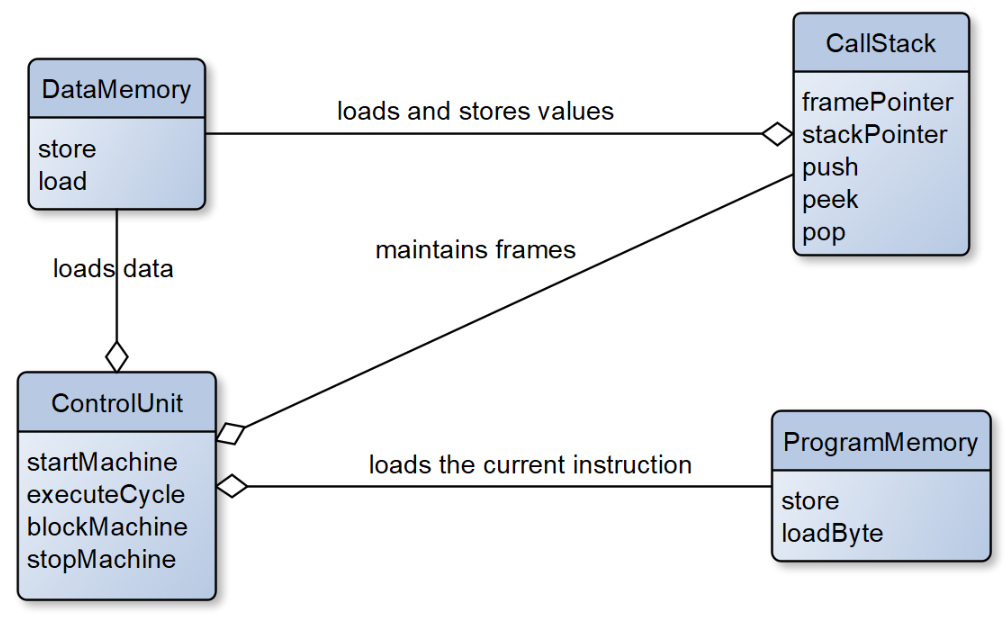
\includegraphics[scale=.62]{images/componentsOfNbM.png}
	\caption{Components of the NoBeardMachine Architecture}
	\label{fig:componentsOfNbM}
\end{figure}
\subsection{Program Memory}
The program memory stores instructions with their corresponding opcodes and operands. The memory is byte addressed with a specified  maximum size. Memory access outside the valid range lead to a \lstinline$ProgramAddressError$.

\subsection{Data Memory} \label{sec:dataMemory} 
The data memory is a byte addressed storage and stores variables as follows:

\begin{itemize}
\item \textbf{Characters} are one-byte values and consume exactly one byte in memory, i.e., no alignment is done. 
\item \textbf{Integers }are four-byte values and stored in little endian order. Negative integer values are stored as Two’s Complement (see \cite{wikipedia_twos_2018}).
\item \textbf{Booleans }are four-bytes values and are stored as the integer 0 for false and the integer 1 for true.
\end{itemize}

\begin{figure}[H]
\begin{center}
\begin{tabular}{p{8em}|p{8em}|}
\cline{2-2}
\parbox[t][3em][t]{8em}{\hfill 0} & String Constants \\[3em] \cline{2-2}
& Stack frame 1 \\[2em] \cline{2-2}
& Stack frame 2 \\[2em] \cline{2-2}
& \ldots \\[2em] \cline{2-2}
\parbox[b][4em][b]{8em}{\hfill MAX\_DATA} & free \\ \cline{2-2}
\end{tabular}
\end{center}
\caption{Data Memory of the NoBeard Machine}\label{fig:datamemory}
\end{figure}

As figure~\ref{fig:datamemory} shows, the data memory is separated into two parts, string constants and to stack frames of the currently running functions. 

\subsubsection{String Constants}
String constants are in the top segment of the data memory. It includes all strings that have to be printed on the console. The storing of string constants happens exactly after the opening of a binary file on the virtual machine. 

\subsubsection{Stack Frames}
After the constant memory the stack frames are maintained. Whenever a function gets called a new frame is added. It holds data for the function arguments, local variables and its expression stack. As soon as a function ends, its frame is removed. 

\begin{figure}[H]
\begin{center}
\begin{tabular}{p{8em}|p{4em}|p{15em}}
\parbox[b][1em][b]{8em}{\hfill \cellcolor{Gray}\textcolor{White}{Address}} & \cellcolor{Gray}\textcolor{White}{Content} & \cellcolor{Gray}\textcolor{White}{Remark} \\ \cline{2-2} 
\cline{2-2}
\parbox[t][1em][t]{5em}{\hfill 0} & 0 & frame pointer of frame 0 \\ \cline{2-2}
& \ldots \\ \cline{2-2}
\parbox[t][1em][t]{5em}{\hfill 32} & 13 & local int in frame 0 \\ \cline{2-2}
\parbox[t][1em][t]{5em}{\hfill 36} & 0 & static link to frame 0 (start of frame 1)\\ \cline{2-2}
& \ldots \\ \cline{2-2}
\parbox[t][1em][t]{5em}{\hfill 68} & 17 & local int in frame 1\\ \cline{2-2}
\parbox[t][1em][t]{5em}{\hfill 72} & 42 & local int in frame 1\\ \cline{2-2}
\parbox[t][1em][t]{5em}{\hfill 76} & 36 & static link to frame 1 (start of frame 2) \\ \cline{2-2}
& \ldots \\ \cline{2-2}
\parbox[t][1em][t]{5em}{\hfill 108} & `D' \\ \cline{2-2}
\parbox[t][1em][t]{5em}{\hfill 109} & 61 \\ \cline{2-2}
\parbox[b][4em][b]{8em}{\hfill MAX\_DATA} & free \\ \cline{2-2}
\end{tabular}
\end{center}
\caption{Snapshot of a call stack with three frames}\label{fig:threeframes}
\end{figure}

Figure~\ref{fig:threeframes} shows a pretty good example from \cite{bauer_p._2017}. Here we can see that the memory is working with three frames. Frame~0 starts at address 0. The first 32 bytes of each frame are reserved for administrative data like the static link and the dynamic link to the surrounding frame, the return value, etc. Address~32 holds the value of a local variable in frame~0.
At address~36 frame~1 starts with the address to its statically surrounding frame, i.e, the function (or unit or block) represented by frame~0 is defining the function (or block) represented by frame~1. Frame~1 defines two local values at addresses 68 and 72. 

\subsection{Call Stack}
By structuring the data memory as a stack the call stack is needed as an abstraction to the data memory. With the help of different functions the call stack is able to add and remove frames from the stack and to maintain the expression stack. Data needed for each statement gets stored in the expression stack. It grows and shrinks as needed and is empty at the end of each NoBeard statement. The stack is addressed word-wise only. Functions like \lstinline$push()$, \lstinline$peek()$ and \lstinline$pop()$ are provided for the maintenance of values on the stack. The call stack has the two major components:

\begin{itemize}
\item \textbf{Stack Pointer: }Address of the start of the last used word on the stack. 
\item \textbf{Frame Pointer: }Address of the first byte of the currently running function's stack frame. 
\end{itemize}

\subsection{Control Unit}
The control unit is responsible for the program work flow. It executes one machine cycle in three steps, it fetches, decodes and operates the current instruction. Depending on some instruction, the control unit also affect the state of the machine. To achieve these steps it has to work with the following components:

\begin{itemize}
\item \textbf{Program Counter: }Start address of the next instruction to be executed.
\item \textbf{Machine State: }The NoBeard machine has four different states and is always in one of them. 
	\begin{itemize}
		\item \lstinline$running$: The machine runs
		\item \lstinline$stopped$: The machine stops. Usually when the end of program is reached.
		\item \lstinline$blocked$: The machine pauses. Mostly when a breakpoint is placed by the user.
		\item \lstinline$error$: Error state
	\end{itemize}
\end{itemize}
As already mentioned the machine has a firmly defined execution cycle:

\begin{enumerate}
\item Fetch instruction
\item Decode instruction
\item Execute instruction
\end{enumerate}

The very first instruction is fetched from a specified starting program counter which is provided as an argument when starting the program. From this point of time onwards the program is running until the machine state changes from run. There are two options to interrupt the machine from running state. First, if it gets interrupted by a breakpoint typically set by the debugger and second, if a \lstinline$halt$ instruction gets executed.

\section{Binary File Format}
The virtual machine runs only NoBeard object files with extension \lstinline$.no$ which can be generated by the NoBeard Assembler or NoBeard Compiler. As figure~\ref{fig:binaryfileformat} shows NoBeard binaries are separated into three parts, a header part, a string storage and a program segment.
The first six bytes are reserved for the header part which holds information about the file. This information includes the file identifier and the version of the file. After the header follows the string storage where a stream of constants are stored. Finally, the program segment which is organized like the string storage deals with the storing of machine instructions. 
\begin{figure}[h]
\begin{center}
\begin{tabular}{p{1em}|p{10em}|}
\cline{2-2}
\parbox[c][3em][t]{1em}{\hfill 0} & Header \\ \cline{2-2}
\parbox[c][4em][t]{1em}{\hfill 6} & String storage \\ \cline{2-2}
\parbox[c][5em][b]{1em}{\hfill N} & Program segment \\ \cline{2-2}
\end{tabular}
\end{center}
\caption{NoBeard Binary File Format}\label{fig:binaryfileformat}
\end{figure}

\section{Instructions}\label{sec:instructions}
NoBeard instructions are of a different length and each has an opcode and operands of an amount between 0 and 2. The first byte of all instructions is reserved for the opcode, which is the identifier used to identify the instruction on machine language level. The remaining bytes, if any, are assigned to the operand(s) of the instruction.
Each of the following subsections explains these instructions in four categories. The underlined title is the shorthand that identifies the instruction on assembler level. Then follows a table showing the size of the instruction and which bytes carry which information. Finally, each one has also a short explanation in human language.

\subsection{Load and Store Instructions}
% ----------------------------- LIT ----------------------------
\subsubsection{lit}
\threebyteinstruction{0x01}{Literal}

\paragraph{Operation:}
Pushes a value on the expression stack.

% ----------------------------- LA ----------------------------
\subsubsection{la}
\fourbyteinstructiona{0x02}{Displacement}{DataAddress}

\paragraph{Operation:}
Loads an address on the stack.

% ----------------------------- LV ----------------------------
\subsubsection{lv}
\fourbyteinstructiona{0x03}{Displacement}{DataAddress}

\paragraph{Operation:}
Loads a value on the stack.

% ----------------------------- LC ----------------------------
\subsubsection{lc}
\fourbyteinstructiona{0x04}{Displacement}{DataAddress}

\paragraph{Operation:}
Loads a character on the stack.

% ----------------------------- LVI ----------------------------
\subsubsection{lvi}
\fourbyteinstructiona{0x05}{Displacement}{DataAddress}

\paragraph{Operation:}
Loads a value indirectly on the stack.

% ----------------------------- LCI ----------------------------
\subsubsection{lci}
\fourbyteinstructiona{0x06}{Displacement}{DataAddress}

\paragraph{Operation:}
Loads a character indirectly on the stack.

% ----------------------------- INC ----------------------------
\subsubsection{inc}
\threebyteinstruction{0x1D}{Size}

\paragraph{Operation:}
Increases the size of the stack frame by \lstinline$Size$.

% ----------------------------- STO ----------------------------
\subsubsection{sto}
\onebyteinstruction{0x07}

\paragraph{Operation:}
Stores a value on an address.

% ----------------------------- STC ----------------------------
\subsubsection{stc}
\onebyteinstruction{0x08}

\paragraph{Operation:}
Stores a character on an address.

\subsection{Integer Instructions}


% ----------------------------- NEG ----------------------------
\subsubsection{neg}
\onebyteinstruction{0x0B}

\paragraph{Operation:}
Negates the top of the stack.

% ----------------------------- ADD ----------------------------
\subsubsection{add}
\onebyteinstruction{0x0C}

\paragraph{Operation:}
Adds the top two values of the stack.

% ----------------------------- SUB ----------------------------
\subsubsection{sub}
\onebyteinstruction{0x0D}

\paragraph{Operation:}
Subtracts the top two values of the stack.

% ----------------------------- MUL ----------------------------
\subsubsection{mul}
\onebyteinstruction{0x0E}

\paragraph{Operation:}
Multiplies the top two values of the stack.

% ----------------------------- DIV ----------------------------
\subsubsection{div}
\onebyteinstruction{0x0F}

\paragraph{Operation:}
Divides the top two values of the stack.

% ----------------------------- MOD ----------------------------
\subsubsection{mod}
\onebyteinstruction{0x10}

\paragraph{Operation:}
Calculates the remainder of the division of the top values of the stack.

% ----------------------------- NOT ----------------------------
\subsubsection{not}
\onebyteinstruction{0x11}

\paragraph{Operation:}
Calculates the remainder of the division of the top values of the stack.

\subsection{Control Flow Instructions}

% ----------------------------- FJMP ----------------------------
\subsubsection{fjmp}
\threebyteinstruction{0x16}{NewPc}

\paragraph{Operation:}
Sets \lstinline$pc$ to \lstinline$newPc$ if stack top value is false.

% ----------------------------- TJMP ----------------------------
\subsubsection{tjmp}
\threebyteinstruction{0x17}{NewPc}

\paragraph{Operation:}
Sets \lstinline$pc$ to \lstinline$newPc$ if stack top value is true.

% ----------------------------- JMP ----------------------------
\subsubsection{jmp}
\threebyteinstruction{0x18}{NewPc}

\paragraph{Operation:}
Unconditional jump: Sets \lstinline$pc$ to \lstinline$newPc$.

% ----------------------------- BREAK----------------------------
\subsubsection{break}
\onebyteinstruction{0x20}

\paragraph{Operation:}
Breaks the machine. Especially used for the debugging function.

% ----------------------------- HALT ----------------------------
\subsubsection{halt}
\onebyteinstruction{0x1F}

\paragraph{Operation:}
Halts the machine.

\subsection{IO-Instructions}

% ----------------------------- IN ----------------------------
\subsubsection{in}\label{sec:in}
\twobyteinstruction{0x19}{Type}

\paragraph{Operation:}
Reads data from the terminal. Depending on \lstinline$Type$ different data types are read:

\begin{itemize}
	\item 0: An \lstinline$int$ is read and stored at the address on top of the stack. After execution the value 1 is pushed if an integer was read successfully, otherwise 0 is pushed.
	\item 1: A \lstinline$char$ is read and stored at the address on top of the stack. After execution the value 1 is pushed 
	\item 2: a \lstinline$string$ with a specific length is read
\end{itemize}

% ----------------------------- OUT ----------------------------
\subsubsection{out}\label{sec:out}
\twobyteinstruction{0x1A}{Type}

\paragraph{Operation:}
Writes data to the terminal. Depending on \lstinline$Type$ different data types are printed:

\begin{itemize}
	\item 0: An \lstinline$int$ with a specific column width is printed
	\item 1: A \lstinline$char$ with a specific column width is printed
	\item 2: a \lstinline$string$ with a specific column width is printed
	\item 3: a new line is printed
\end{itemize}
	
\section{NoBeard Assembler}
To write programs for the NoBeard machine an Assembler is provided. NoBeard Assembler files are separated in two blocks, which is called the string constants and the assembler program. The files have the extensions \lstinline$.na$ for NoBeard Assembler. The string constants are stored between two double quotes and has to be located at the beginning of the file. There is no way to address a single constant. So, if we use a string constant in the assembler program, we have to specify the starting address of the string constant and the length needed in the program. Assembler programs  contain a sequence of assembler instructions like \lstinline$lit$ for load or \lstinline$out$ for print. After the opcode of the instruction follows the operands, if they are needed as already described in section \ref{sec:instructions}.
\chapter{User Manual}
\lstset{language=NoBeardAsm}
\section{Overview}
This chapter describes how to use the graphical user interface of the NoBeard virtual machine and serves at the same time as a user manual. With the NoBeard Machine users are able to load and run NoBeard object files with just a view clicks. The integrated debugger of the virtual machine gives them also the possibility to debug these programs by setting breakpoints and stepping through the program in one by one assembler instructions. Another big feature is the data visualization which gives users a whole view of the data memory.
\section{The UI Components}
As shown in figure~\ref{fig:components} the NoBeardMachine contains the following five windows:

\begin{figure}[h] 
	\centering
	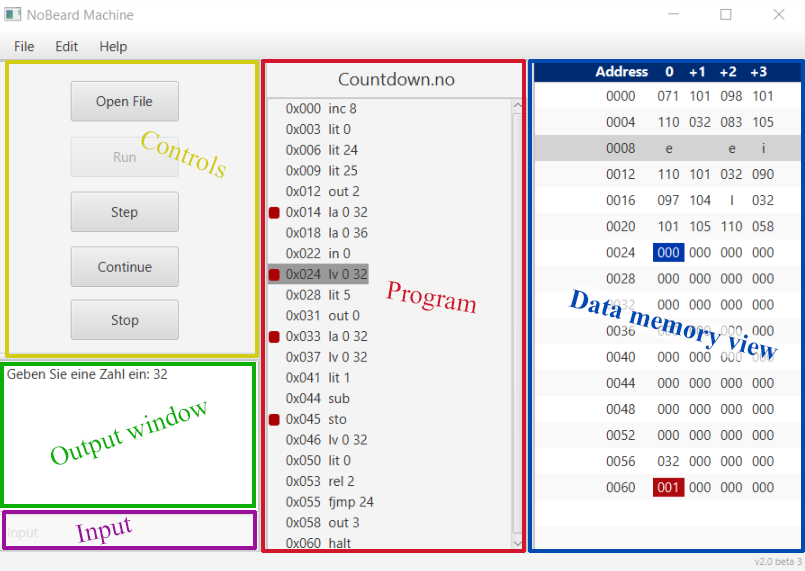
\includegraphics[scale=.87]{images/screenshot-0.png}
	\caption{Components of the NoBeardMachine}
	\label{fig:components}
\end{figure}

\begin{itemize}
\item \textbf{Control Window: }A window with a set of buttons for user interactions.
\item \textbf{Output Window: }A terminal showing outputs of programs and user inputs.
\item \textbf{Program Window: }Shows the actually opened program and its running flow.
\item \textbf{Data Memory Window: }A visualized call stack of a debugged program.
\item \textbf{Input Window: }A single-line field for user inputs.
\end{itemize}

\subsection{Control Window}
This window consists of five buttons that gives the possibility to open, run, stop programs, step between instructions or continue execution from a breakpoints until another one. 
\begin{itemize}
\item \textbf{Open file: }Opens a file chooser dialog where the target object file can be selected.
\item \textbf{Run: }Executes the program from the first instruction. 
\item \textbf{Step: }Allows the user to step one single assembler instruction further in the program flow. This button is only enabled if the machine is in state \lstinline$blocked$.
\item \textbf{Continue: }When the program execution gets interrupted by a breakpoint this button enables users to continue the execution of the program until the next breakpoint or the end of the program. If there is no breakpoints left it continues the process until the end.
\item \textbf{Stop: }Stops the execution and sets the machine into the \lstinline$stopped$ state.
\end{itemize}
\subsection{Output Window}
The output window is a non-editable text area which simulates a terminal. Program outputs that are coming from a NoBeard \lstinline$out$ instruction are shown here. Submitted inputs are also visible here after a successful submit.
\subsection{Program Window}
The program window shows the assembler instructions of the loaded program with the corresponding start address of each instruction. When clicking on the empty area in front of the instruction's address a breakpoint can be set or unset.  
\subsection{Data Memory Window}
A ListView filled with raw data from the data memory. Every line of the ListView contains four byte data with the belonging addresses. The raw data can be converted into different formats like characters or integers to make it better readable to humans. Furthermore the frame pointer and the stack pointer of the currently running frame are highlighted. Each byte can be converted to a character and a whole line can be translated to four characters or to a single four byte integer. Data with blue background color highlights the frame pointer. Red background color stands for the stack pointer.
\subsection{Input Window}
The Input window is a TextField where inputs from users can be handled. It is only enabled when the machine is executing an \lstinline$in$ instruction. To submit an input, the "ENTER" key has to be pressed and then the entered text will be attached to the Output window.

\section{Loading and Running a Program}
After starting the NoBeardMachine, a NoBeard object file has to be loaded by a click on the “Open File” button. Than a file chooser dialog appears where the user can choose the desired file. Afterward the window shows the assembler code and the title of the opened program which is now ready for execution.

The Program window lists the assembler instructions with the belonging operators and addresses in decimal form. By hitting the “Run” button, the machine executes the loaded program. Output results can be seen in the Output window. If the program runs against an input instruction, the machine stops and requests the user for an input which can be done at the Input window. To submit an input, the Enter key has to be pressed. After the user pressed the Enter key the program continues its execution.
\begin{figure}[h] 
	\centering
	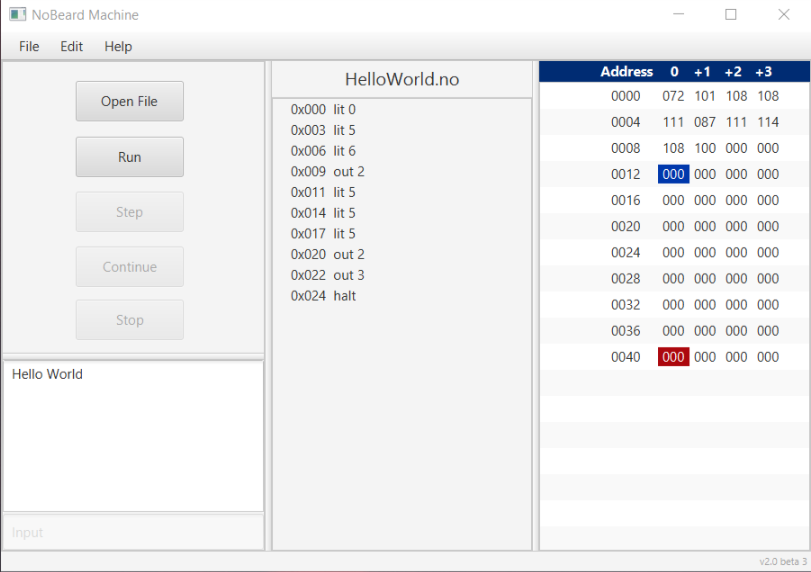
\includegraphics[scale=.85]{images/screenshot-1.png}
	\caption{Executed "Hello World" program}
\end{figure}

\section{Debugging}
To debug a program the user has to set breakpoints which interrupts the program flow and allows the user to inspect the current state of the running program. These breakpoints can be placed by clicking on the address or onto the empty space in front of the address with the instruction where the program flow has to be interrupted. 

After an interruption caused by a breakpoint, the user is able to step one line further or continue execution until to the next breakpoint. Stepping is handled by the “Step” button as shown in figure~\ref{fig:debugging}. By clicking the “Continue” button, the program runs from the current line until the next breakpoint. If there is not any breakpoint left from the current line, it runs until the end of the program. Optionally, the user is able to stop the program during the execution. This could be achieved by clicking the “Stop” button.
\begin{figure}[h] 
	\centering
	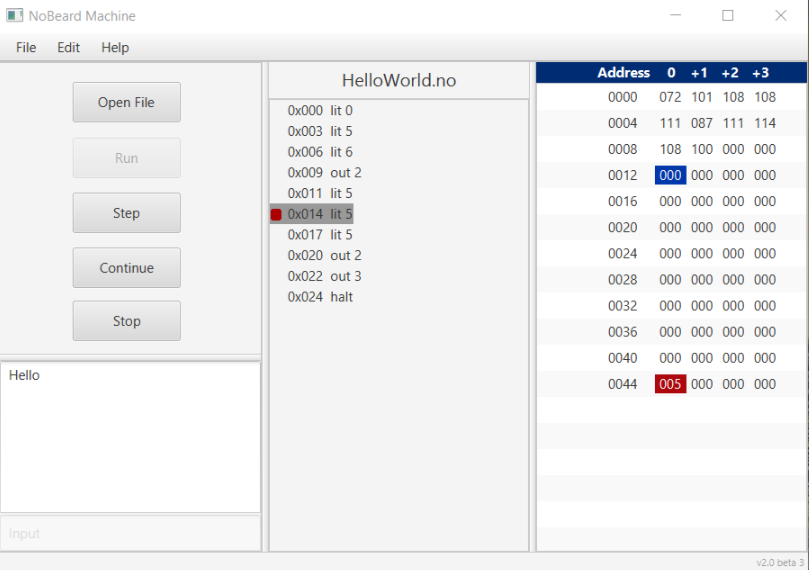
\includegraphics[scale=.85]{images/screenshot-2.png}
	\caption{Debugging the "Hello World" program}
	\label{fig:debugging}
\end{figure}

\section{Data Visualization}
On the right side of the window is the visualisation of the data memory in a ListView form. This window lists data byte-wise from the data memory of the machine. Each line of the ListView has a content of an address given in decimal notation followed by four bytes of raw data. The memory is separated in two parts. The list starts on the top with the string constants followed by stack frames of the currently running functions. While the frame pointer is highlighted with a blue background, the stack pointer is signed with a red background. The user has also the possibility to convert raw data to characters or integers.
With a right click on the selected line of the list, a context menu opens. The context menu includes the following functions which will be described in the sections thereafter:
\begin{itemize}
\item Converting a single byte to character or a whole line to four characters
\item Converting data to integer 
\item Converting a line back to raw data. 
\end{itemize}
\begin{figure}[h] 
	\centering
	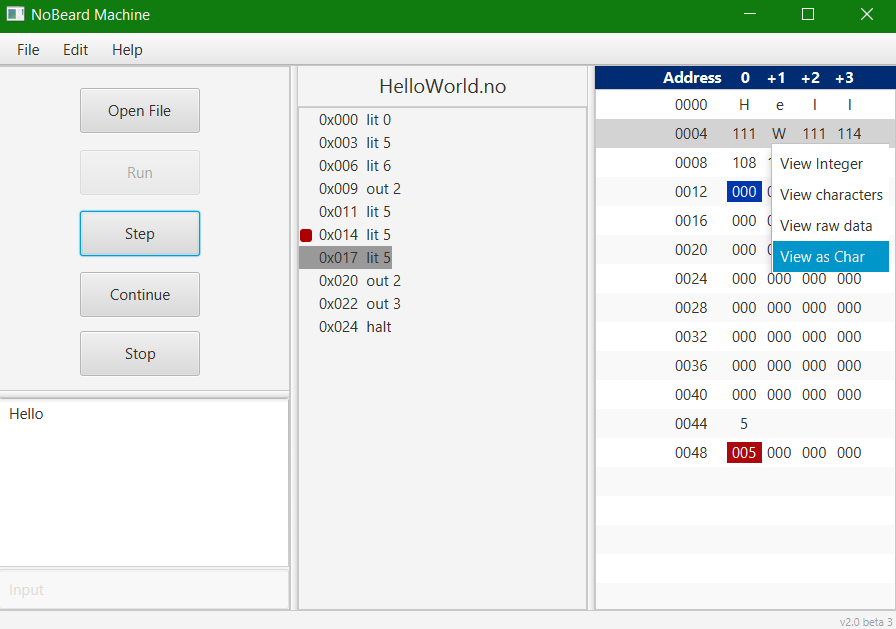
\includegraphics[scale=.80]{images/screenshot-3.png}
	\caption{Converting data to a character}
	\label{fig:convertToChar}
\end{figure}
\subsection{Converting Data to Character}
To view a character of a one-byte data as shown in figure~\ref{fig:convertToChar}, the following steps have to be done:
\begin{enumerate}
\item Select the line where the one-byte value is located 
\item Right click on the value to be converted
\item Click on "View as Char" 
\end{enumerate}
Now the value at the given address is translated to an alphanumeric character. 
The conversion of an entire row of data to characters is done in the same way except that the user has to click "View characters" instead of "View as Char"
\subsection{Converting Data to Integer}
The translation of an integer takes four bytes that means, it takes four data cells from the desired start address and translates them to a single integer.  
\begin{figure}[h] 
	\centering
	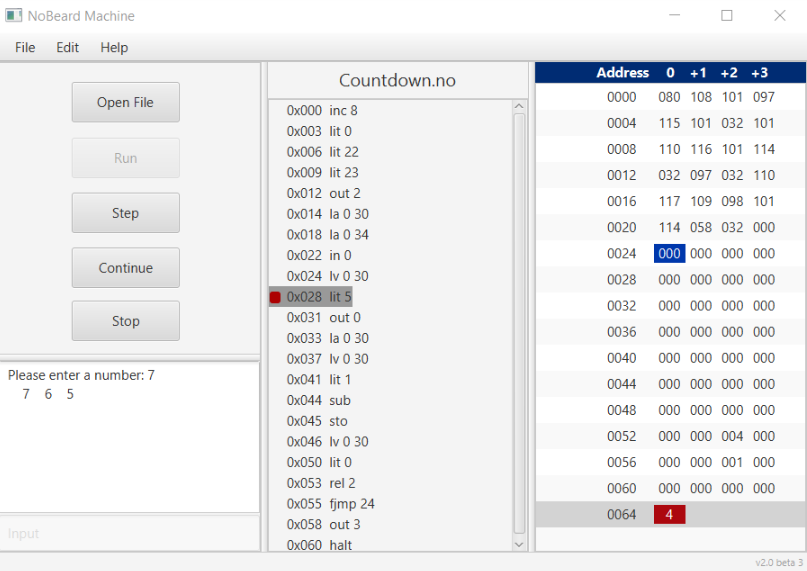
\includegraphics[scale=.90]{images/screenshot-4.png}
	\caption{Converting four-byte data to a single integer}
	\label{fig:convertToInt}
\end{figure}
\begin{enumerate}
\item Select the data cell with the start address of the integer
\item Right click on the cell
\item Click on "View Integer"
\end{enumerate}
After a successful conversion, the four data cells are being replaced by a single integer. Figure~\ref{fig:convertToInt} shows an example of the translated integers. The first one is at address 54 which is not aligned in one row and the second one is on the same place as the stack pointer, precisely at the address 64. 

\subsection{Multiple Conversion}
To facilitate the conversion from raw data to alphanumeric characters a multi selection function is available for the list of the data memory.
To convert multiple data rows, the user has to hold the "Ctrl" key and select the specified rows with a left mouse click. Chosen lines will get highlighted with a light grey background color. As figure~\ref{fig:multipleConversion} shows, the selected rows with grey background are successfully concerted to some characters.
\begin{figure}[h] 
	\centering
	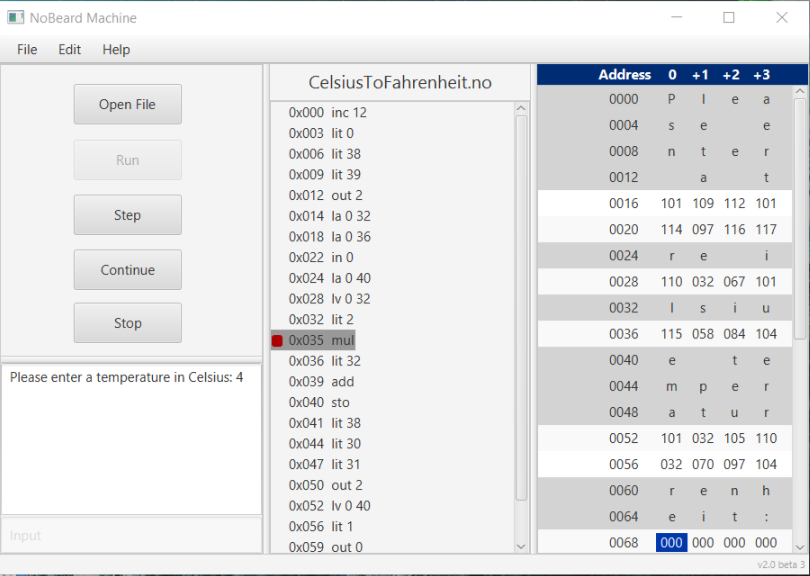
\includegraphics[scale=.85]{images/screenshot-5.png}
	\caption{Multiple conversion of data}
	\label{fig:multipleConversion}
\end{figure}

\chapter{Implementation}
\lstset{language=NoBeardAsm}
\section{Used Technologies}
\subsection{IntelliJ IDEA} 
The implementation of the project is written in Java using the integrated development environment IntelliJ IDEA which is mainly for developing Java based software. Nevertheless, it supports other programming languages too like Scala, Groovy, Kotlin etc\ldots It also support PHP, HTML, CSS3, JavaScript and TypeScript that could be very practicable for web development with the combination of different frameworks like AngularJs, Node.js, SQL Server etc… Another big advantage that IntelliJ IDEA has is the mobile development in Android or Cordova. 
This IDE support a huge variety of benefits such as:
\begin{itemize}
\item Different build systems (maven, gradle, ant, grunt, bower, etc \ldots)
\item Version control systems (Git, Mercurial, Perforce, and SVN)
\item Plugin ecosystem
\item Test runner and coverage
\end{itemize}
More about this topic can be found on this site: \cite{intellij_intellij_nodate}

\subsection{Maven} 
This is a software management and build automation tool which is based on the concept of a project object model (POM). POM is fundamental unit of work in Maven. It is an XML file that resides in the base directory of the project as pom.xml.
The POM contains information about the project and various configuration detail used by Maven to build the project(s).
POM also contains the goals and plugins. While executing a task or goal, Maven looks for the POM in the current directory. It reads the POM, gets the needed configuration information, and then executes the goal. 

One of the biggest features in Maven is the dependency management. Maven automatically downloads the libraries and plug-ins declared in the POM file from the Maven central repository and stores them locally. In simple, when a developer builds a Maven project, all dependency files will be stored in a Maven local repository. So if Maven finds dependency libraries in the Maven local repository, it do not need to download them from the default online Maven central repository multiple time.

By default, the local Maven repository is the .m2 folder
\begin{itemize}
\item \textbf{Unix/Mac OS X: }\lstinline$~/.m2$
\item \textbf{Windows: }\lstinline$C:\Users\{your-username}\.m2$
\end{itemize}

The Maven command \lstinline$mvn install$ builds a project and places its binaries in the local repository. Then other projects can utilize this project by specifying its coordinates in their POMs. Further information about Maven can be found on the official website: \cite{maven_maven_nodate}

\subsection{JavaFX}
JavaFX is a framework which enables developers to design rich client applications that is able to run constantly on different platforms. It offers a wide range of APIs for web rendering, user interface styling and media streaming. JavaFX relies in particular on a scene graph, which manages the individual components of a GUI. It also provides a declarative description of XML-based graphical interfaces with FXML.

The newest JavaFX releases are fully integrated with the current Java SE Runtime Environment(JRE) and Java Development Kit(JDK), which is available for all main desktop platforms. 
More about this topic can be found on the following website: \cite{javafx_main_nodate}

\subsection{Scene Builder} \label{sec:SceneBuilder}
JavaFX Scene Builder is a visual layout tool that generates FXML, an XML-based markup language that lets developers quickly design user interfaces, without any coding. Users just have to drag and drop UI components to the work area. By selecting components users can easily modify their properties or apply style sheets. The XML code for the layout is generated automatically in the background by the tool.

The resulting FXML file can be combined with a Java project by binding the UI to the application’s logic. Every item of the layout view can be assigned with an fx:id to give the controller an easy access of components by the ``@FXML'' annotation. SceneBuilder is an external tool so it has to be downloaded from the official Oracle website and has to be integrated to a Java supporting IDE. 
More about this topic can be found on its website: \cite{scenebuilder_javafx_nodate}

\section{Supporting NoBeard Packages}
The NoBeard Machine is part of the existing NoBeard project. This project already consists of the following packages:
\begin{itemize}
\item \textbf{asm: }NoBeard Assembler to assemble .na files 
\item \textbf{compiler: }NoBeard Compiler to compile .nb source code files
\item \textbf{config: }Hold information of the NoBeard project
\item \textbf{error: }To handle errors that are occurring during compilation or assembly   
\item \textbf{io: }Responsible for reading source files and handling binary files 
\item \textbf{machine: }Implements a virtual machine with components like DataMemory, ProgramMemory, Instructions, etc...  
\item \textbf{parser: }Converts source code files to binary files \bau{This has to be done better after you have done the introductory chapters}
\item \textbf{scanner: }To analyze NoBeard source code files for keywords, operands or arguments  \bau{see above}
\item \textbf{symbolTable: }Looks up for matching words based on the symbol table entry  \bau{see above}
\end{itemize}
However, the most important package for our work is \lstinline$machine$. It defines the interface which the project described here is built upon.
\section{Architecture of the User Interface}
This is the model view controller pattern. The model is responsible for holding data. In our case this is not in a data base but the data is held in the virtual machine. The Model-View-Controller pattern does not require necessarily a database.

The GUI project is build up of three main components as shown in figure~\ref{fig:partsOfGui}. The Controller and the Virtual Machine both of them are running on different threads and are accordingly synchronized. This will be described in detail in section~\ref{sec:synchronization}. The relationship between the controller and view is for event actions and updating of view-components like data memory, output or program flow. The View allows users to call functions from the Controller by clicking on control buttons or by entering inputs. 
\begin{figure}[h] 
	\centering
	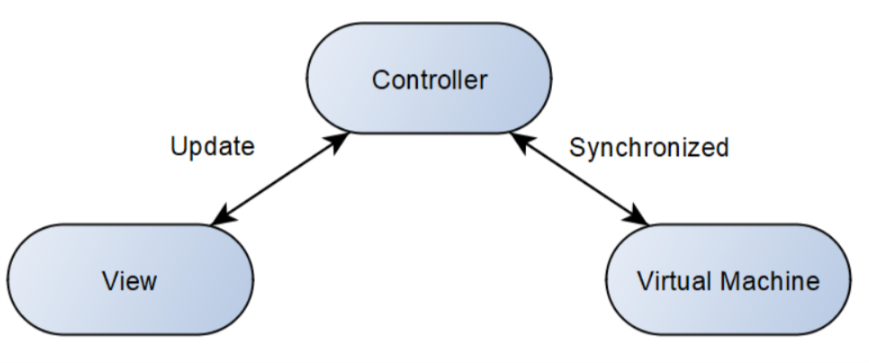
\includegraphics[scale=.70]{images/modelOfGui.png}
	\caption{Main parts of the GUI implementation}
	\label{fig:partsOfGui}
\end{figure}
\subsection{The View}\label{sec:TreeView}
The view is basically a single \lstinline$.fxml$ file which holds the view components of the layout. As figure~\ref{fig:view} shows it was created with an external tool called Scene Builder which is already described in section~\ref{sec:SceneBuilder}.

Each window is made up of an \lstinline$AnchorPane$ \cite{anchorpane_anchorpane_nodate} and is separated by \lstinline$SplitPanes$. An \lstinline$AnchorPane$ enables developers to build flexible user interfaces which can adapt automatically to different screen sizes and orientations. It provides the possibility to constrain the position and size of each element to its parent or siblings. So it becomes very comfortable and easy to size every window as the user wants. Very similar concepts are available in other UI frameworks as Android (\lstinline$LinearLayout$ \cite{android_linearlayout_nodate}) or iOS (\lstinline$UIStackView$ \cite{apple_uistackview_nodate}).

Then each of these \lstinline$AnchorPane$s holds the needed view-components like \lstinline$Button$, \lstinline$TextArea$, \lstinline$TextField$, \lstinline$ListView$ or \lstinline$ScrollPane$.

There are two types of designing and both of them is used in this project to develop a UI that meets all usability requirements.

\subsubsection{Static Design}
Static designing means that all view components are defined in the layout file and not in the Java code. With this type of designing it is pretty easy to build quickly a basic user interface. The developer has only to define the components in an fxml file or place them onto the view via drag and drop with the help of Scene Builder. This part of a project is mostly done by a designer because it does not require a lot of programming knowledge. Listing~\ref{listing:XmlCode} shows a simplified version of how the control buttons were defined in the fxml file.
\lstset{language=XML,style=MyStyle}
\begin{lstlisting}[caption={FXML example}, label=listing:XmlCode]
<AnchorPane>
	<Button fx:id="openButton" onAction="#openFile" text="Open File"/>
	<Button fx:id="startButton" onAction="#startProgram" text="Run"/>
	<Button fx:id="stepButton" onAction="#step" text="Step"/>
	<Button fx:id="continueButton" onAction="#continueToBreakpoint" text="Continue"/>
	<Button fx:id="stopButton" onAction="#stopProgram" text="Stop"/>
</AnchorPane>
\end{lstlisting}

\subsubsection{Dynamic Design}
In dynamic design the already existing view-components is being changed according to run time conditions or to user interactions. This means that the content of statically placed controls changes e.g., by filling or updating a table view. Another typically dynamic designing is when the appearance of these items gets altered through enabling a button or changing its text. This is usually when a user or system triggers an event that matches a particular condition. In this case, the design code has to be mixed with the Java code and therefore programming skills from both sides are necessary. 

Code snippet~\ref{listing:ProgramDataView} shows the \lstinline$fillProgramDataView$ function which is called after a user opens a binary file. This function fills the program window with the content and additionally inserts a \lstinline$CheckBox$ to each line for maintaining the breakpoints.

\lstset{
  language=Java,
  identifierstyle=\color{black},
  keywordstyle=\color{blue},       % keyword style
  stringstyle=\color{forestgreen},     % string literal style
}
  
\begin{lstlisting}[caption={Implementation of program data view},label=listing:ProgramDataView]
private void fillProgramDataView(List<String> programDataList) {
    VBox programData = new VBox();
    for (String lineStr : programDataList)
        addLineToProgramDataView(programData, lineStr);
    programDataView.setContent(programData);
}

private void addLineToProgramDataView(VBox programData, String lineContent) {
    CheckBox line = new CheckBox(lineContent);
    line.setPadding(new Insets(1));
    line.setOnAction((event) -> setClickEventToLine((CheckBox) event.getSource()));
    programData.getChildren().add(line);
    programDataMap.put(getAddressOfProgramLine(line.getText()), line);
}

private void setClickEventToLine(CheckBox breakpoint) {
    if (breakpoint.isSelected())
        machine.addBreakpoint(getAddressOfProgramLine(breakpoint.getText()));
    else
        machine.removeBreakpoint(getAddressOfProgramLine(breakpoint.getText()));
}
\end{lstlisting}

\begin{figure}[h] 
	\centering
	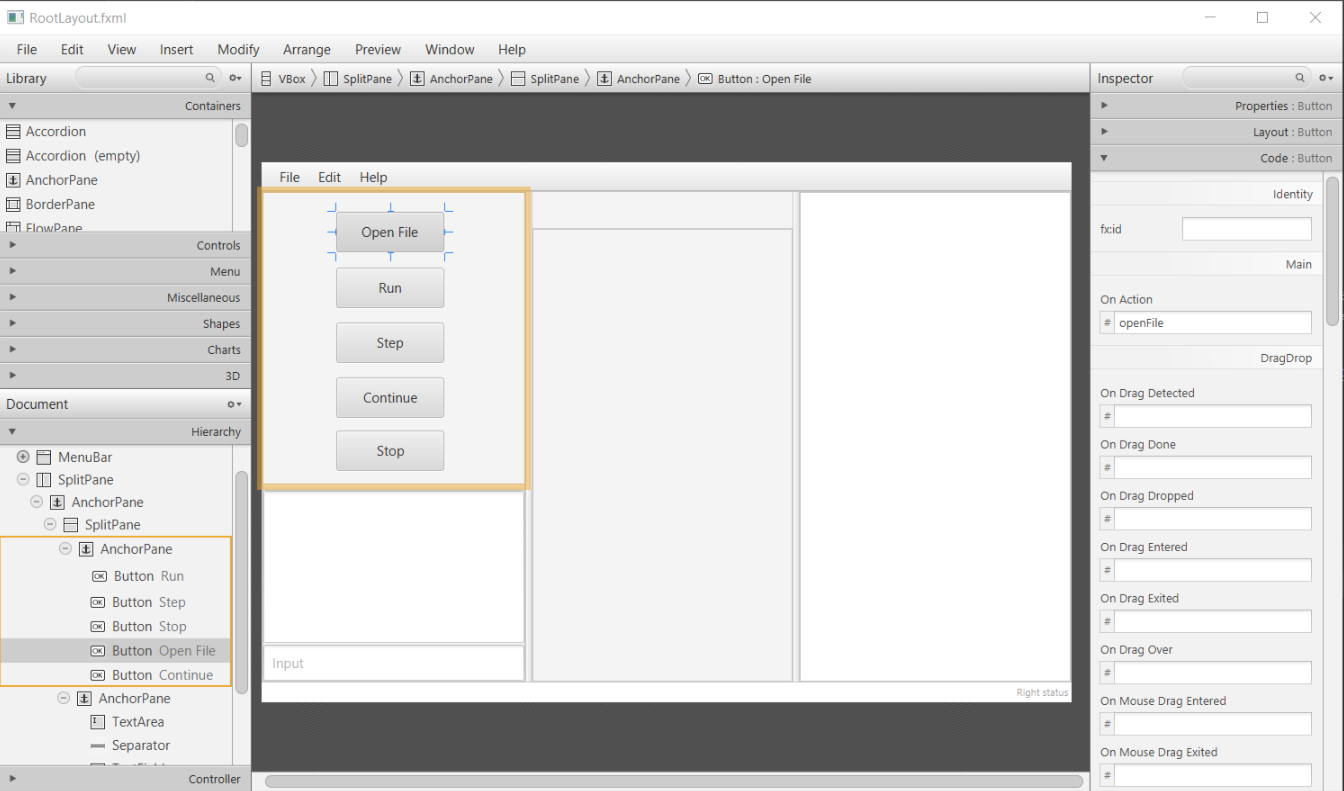
\includegraphics[scale=.55]{images/view.png}
	\caption{Development of the view with Scene Builder}
	\label{fig:view}
\end{figure}
\subsection{The Controller}
The controller is primarily responsible for the coordination and operation of the view and its components. As already described in section~\ref{sec:SceneBuilder} the controller gets access to the view components via the binding of an fx id. To enable this access the view and the controller have to be connected by setting the \lstinline$fx:controller$ attribute of the root view element to the currently used controller. The user interface defined by an FXML file and its controller is loaded into memory by an \lstinline$FXMLLoader$. When the \lstinline$load()$ method is called on the \lstinline$FXMLLoader$, it:
\begin{enumerate}
\item Loads the FXML file
\item Creates an instance of the controller class specified by the \lstinline$fx:controller$ attribute, by calling its no-argument constructor
\item Sets the value of any @FXML-annotated fields in the controller to the elements defined with matching fx:id attributes
\item Registers any event handlers mapping to methods in the controller
\item Calls the \lstinline$initialize()$ method on the controller, if there is one.
\end{enumerate}

Through this advantage event actions like mouse clicks or key presses can be bound between the controller and the view. This could be achieved by setting a name for the ``On Action'' property in Scene Builder and then creating the related function in the controller. The function has to be declared with an \lstinline$@FXML$ annotation and the same name as it was set on the action property of the item.

These action methods accept a single argument of type \lstinline$ActionEvent$. This can be used to get some further information of the fired event like which mouse button was pressed.

Those events have a defined order. The constructor is called before the \lstinline$@FXML$-annotated fields are injected, but the \lstinline$initialize()$ method is called after. This means we can access (and configure) \lstinline$@FXML$-annotated fields in the \lstinline$initialize()$ method, but not in the constructor. It is quite common (at least in simple applications) not to define any constructor in the controller classes.

The other task the controller has to handle is to update the model, i.e., in our case to change the state of the NoBeard machine according to the user commands. So it acts like a bridge to the machine and calls functions like \lstinline$runProgram(int startPc)$, \lstinline$step()$, \lstinline$getCallStack()$ etc\ldots

To achieve this connection between the two components, the controller gets an instance of the NoBeard machine which is being target for NoBeard assembler programs. This happens directly in the \lstinline$initialize()$ method. As said before this method is called automatically and as first when the FX application starts. So every stuff that is needed for the initialization e.g., enabling or disabling controls on the view, is done in this \lstinline$initialize()$ method.

Since the initialization, all other methods can only be invoked by triggering an event like clicking on the ``openFile'' button. However, these event methods gets called under certain conditions that depend on the user. For example, the user has to stop a running program before opening another NoBeard object file. This conclusion gives the controller a defined cycle that the user can execute:
\begin{enumerate}
\item Open file
\item Disassemble file
\item Update view
\item Start program
\end{enumerate}

The opening of a NoBeard object file is operated with the help of a BinaryFileHandler. After an object file is successfully read and program data is available as a binary byte stream it has to be disassembled i.e., that it has to be converted from its binary form to a human readable assembler form.

After this translation is finished the machine has to load the string constants and the program data from the object file into the corresponding memory. Program data is filled in a VBox where each line consists of a CheckBox and an Assembler statement. All of the CheckBoxes get an OnAction event which toggles breakpoints of the machine. This is already demonstrated with the listing~\ref{listing:ProgramDataView}.

When a program is started, a new external thread must be started in which the machine is running separately from the UI. The code~\ref{listing:startingThread} illustrates how the machine gets started on a background thread using a lambda expression.
\begin{lstlisting}[caption={Starting the machine on a new thread},label=listing:startingThread]
@FXML
void startProgram(ActionEvent event) {
    prepareGuiForProgramStart();
    new Thread(() -> {
        machine.runProgram(0);
        highlightNextInstructionToBeExecuted();
        Platform.runLater(() -> DataMemoryView.update(this, getRawDataMemoryList()));
    }).start();
}
\end{lstlisting}
The reason why and how they run on different threads will be explained in section~\ref{sec:synchronization}. The machine executes step by step every instruction of the program until any interruption. It can be interrupted by a breakpoint, input request or by a \lstinline$halt$ instruction. 

The method \lstinline$highlightNextInstructionToBeExecuted()$ at line~6 signs the instruction which hast to be executed as next, e.g., if the user press the ``Step'' button then the highlighted assembler statement will be executed. In other words, it shows where the current program counter is.

The final statement in this code snippet is at line~7 which updates the data memory on the view after an interruption. \lstinline$Platform.runLater(java.lang.Runnable runnable)$ is usually used for updating the GUI from a background thread. Java supports \lstinline$Task$ which is a similar concept and can be utilized for the same purpose. The method \lstinline$DataMemoryView.update$ sets the data memory to the current state, but this will be described in section~\ref{sec:implementationOfDataVisualisation}.

\section{Synchronization of NoBeard Machine and GUI}
\label{sec:synchronization} 
As already mentioned, the NoBeard virtual machine has to run on a background thread. The main reason for this is that there are two different processes using common processing resources. For instance, if they run on the same thread then the user would not be able to make any interactions because the virtual machine locks the main thread. But, even when the virtual machine gets an extra thread there would be still a deadlock because the background thread has to synchronize with the UI thread. So e.g., every time the user has to operate an input, a switch to the UI thread is needed. Otherwise it would cause a critical section between the threads. 

The synchronization of these two threads is implemented with the semaphore construction. A semaphore has a pretty simple usage to solve critical section problems and to achieve process synchronization in the multi processing environment. It is a variable that acts like a traffic light with its \lstinline$acquire()$ and \lstinline$release()$ functions.

The NoBeard Machine contains two interfaces to optimize outputs and inputs on the used device. As soon as the machine executes an input instruction \lstinline$in$, it calls firstly a function from the input interface either \lstinline$hasNextInt()$ or \lstinline$hasNext()$. Both do the same thing, checks whether there is an input by the user or not. The only different is that the one of them also checks if the string is numeric. These functions are overridden in the \lstinline$FxInputDevice$ class where also an instance of the controller is loaded by the constructor. So, by calling one of these \lstinline$hasNext$ function the machine thread should be paused as shown in the code snippet~\ref{listing:Synchronisation1}. To avoid the deadlock, the semaphore from the controller is acquired at this position i.e., at line~11.
\begin{lstlisting}[caption={Synchronisation with semaphore (Part 1)},label=listing:Synchronisation1]
@Override
public boolean hasNextInt() {
    waitForInput();
    return controller.getInput().chars().allMatch( Character::isDigit );
}

private void waitForInput() {
    try {
        controller.enableInputView(true);
        controller.getSemaphore().acquire();
    } catch (InterruptedException e) {
        e.printStackTrace();
    }
}
\end{lstlisting}
Now the user can make an input on the UI thread and submit it. To get back to the machine thread, the semaphore hast to be released after the user fires the submit event by pressing the ENTER key. This is demonstrated with the code fragment~\ref{listing:Synchronisation2} more precisely at line~12. Then the machine continues at the same position where the semaphore was acquired, at one of the has Next function and can analyse the provided input string.
\begin{lstlisting}[caption={Synchronisation with semaphore (Part 2)},label=listing:Synchronisation2]
inputView.setOnKeyPressed(event -> {
    if (event.getCode() == KeyCode.ENTER && inputView != null && 
    !inputView.getText().isEmpty())
        inputIsAvailable(inputView.getText());
});

private void inputIsAvailable(String providedInput) {
    getOutputView().appendText(providedInput + "\n");
    input = providedInput;
    inputView.clear();
    enableInputView(false);
    getSemaphore().release();
}
\end{lstlisting}
\section{Handling of Breakpoints}
Machine internal handling of breakpoints is done as described in \cite{bendersky_how_nodate}. The implementation for the maintaining of breakpoints is coded with a simple observer pattern design to keep the best performance of the virtual machine. 

The idea of this solution is pretty easy to understand. The machine runs only as long as it is in a \lstinline$running$ state. So, a new instruction is introduced, called \lstinline$break$ which sets the machine into a \lstinline$blocked$ state. This means at the same time that as soon as a user sets a breakpoint on a specified instruction, a change from the original to a \lstinline$break$ instruction is necessary.

The \lstinline$ControlUnit$ which is responsible for execution cycles in the virtual machine is going to be an observable class. Then a new Observer class is implemented which is called \lstinline$Debugger$ that is holding all breakpoints in a \lstinline$HashMap$.

\lstinline$private HashMap<Integer, Byte> breakpoints;$
 
This \lstinline$HashMap$ stores the address and the instruction of a selected breakpoint. The \lstinline$Debugger$ class contains in all three major functions as shown in the code snippet~\ref{listing:debugger}. Adding and removing breakpoints to or from the \lstinline$HashMap$ and replacing an instruction at a specified address from the program memory to a new one. The selection of a breakpoint on the UI calls the set or remove function from the debugger, as the case may be. As soon as a breakpoint is selected, it will be stored to the \lstinline$HashMap$ with its original instruction and at same time replaces the original instruction by the newly added \lstinline$break$ instruction.
\begin{lstlisting}[caption={Implementation of the debugger},label=listing:debugger]
void setBreakpoint(Integer address, Byte instructionId) {
    this.breakpoints.put(address, instructionId);
    programMemory.replaceInstruction(address, InstructionSet.Instruction.BREAK.getId());
}

void removeBreakpoint(Integer address) {
    programMemory.replaceInstruction(address, breakpoints.get(address));
    this.breakpoints.remove(address);
}

public void replaceInstructionAtAddress(int address, InstructionSet.Instruction instruction) {
    if (!breakpoints.isEmpty() && breakpoints.keySet().contains(address)) {
        if (instruction != null)
            programMemory.replaceInstruction(address, instruction.getId());
        else
            programMemory.replaceInstruction(address, breakpoints.get(address));
    }
}
\end{lstlisting}
This break instruction sets the machine to a \lstinline$blocked$ state and notify the observer to change the \lstinline$break$ instruction back to the original one which is stored in the \lstinline$HashMap$. 

Now the machine is blocked at a specified breakpoint and the user can take a look to the current stack frames and go one step further in the program or continue the execution cycle to a next breakpoint. However, when the user wants to step further to execute the current instruction where the breakpoint is, of course again a switch back to the break instruction is needed after the original instruction completed.  
\section{Visualisation of DataMemory}
\label{sec:implementationOfDataVisualisation}
The visualisation of the data memory gives an overview about string constants and stack frames. As figure~\ref{fig:dataMemoryView} shows the view lists four byte of data on each row starting with the belonging address. 

Logically, the list has to be updated after any interruption by a breakpoint. This is demonstrated with the code snippet~\ref{listing:startingThread}, more precisely at line~7.

\begin{figure}[h] 
	\centering
	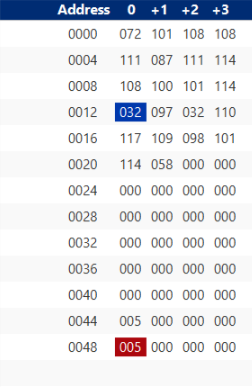
\includegraphics[scale=.99]{images/dataMemory.png}
	\caption{Visualisation of data memory}
	\label{fig:dataMemoryView}
\end{figure}

For the visualisation of these data a \lstinline$ListView$ is defined on the view which is one of the best choice for this purpose. 
The updating of data memory view has defined a cycle. Firstly a function iterates through the memory until the current stack pointer and groups all data into four bytes and finally stores them into an observable collection of strings. Then this collection is assigned to \lstinline$ListView$ items that are visible on the view. Each row of the \lstinline$ListView$ contains now a line of string filled with the address and four pure data. 

Since each item in a \lstinline$ListView$ is represented by an instance of the \lstinline$ListCell$ class, a row can be customized to get a nice structure like in figure~\ref{fig:dataMemoryView}. This customisation of a cell can be achieved with the \lstinline$cellFactory$ API. The cell factory is called by the platform whenever it determines that a new cell needs to be created. 
To specialize the \lstinline$Cell$ used for the \lstinline$ListView$, an implementation of the \lstinline$cellFactory$ callback function has to be provided.
\begin{lstlisting}[caption={Implementation of the data memory view using cell factory},label=listing:CellFactory]
static void update(Controller controller, ObservableList<String> content) {
    controller.getDataMemoryListView().setItems(content);
    controller.getDataMemoryListView().setCellFactory(list -> new ListCell<String>() {
        int framePointer = controller.getMachine().getCallStack().getFramePointer();
        int stackPointer = controller.getMachine().getCallStack().getStackPointer();
        static final int INDEX_OF_ADDRESS = 0;

        @Override
        protected void updateItem(String item, boolean empty) {
            super.updateItem(item, empty);
            if (item != null) {
                createDataLine(item);
            }
        }

        private void createDataLine(String item) {
            HBox line = new HBox();
            int firstAddressInLine = getIndex() * 4;
            convertStringToLabels(firstAddressInLine, item).forEach(line.getChildren()::add);
            setContextMenuToDataCells(line);
            setGraphic(line);
        }

        private List<Label> convertStringToLabels(int firstAddressInLine, String line) {
            String[] lineContent = splitDataLine(line);
            List<Label> result = createLabelForAddress(lineContent[INDEX_OF_ADDRESS]);
            int currentAddress = firstAddressInLine;
            for (int i = 1; i < lineContent.length; i++) {
                if (currentAddress == framePointer)
                    result.add(createHighlightedLabel(lineContent[i], "#0038AC"));
                else if (currentAddress == stackPointer)
                    result.add(createHighlightedLabel(lineContent[i], "#AC080E"));
                else
                    result.add(createNormalLabel(lineContent[i]));
                currentAddress++;
            }
            return result;
        }
        ...
\end{lstlisting}

In the code example~\ref{listing:CellFactory} an anonymous inner class is created using lambda expression, that simply returns instances of \lstinline$ListCell$ overriding the \lstinline$updateItem$ method. This method is called whenever the item in the cell changes, for example when the user scrolls the \lstinline$ListView$ or the NoBeard machine updates the data memory (and the cell is reused to represent some different item in the \lstinline$ListView$). Because of this, there is no need to manage bindings - simply reacting to the change in items when this method occurs. In this example, whenever the item changes, we update the cell text property, and also modify the text fill to ensure that we get the correct visuals.
So each row of the list view will be separated in five labels, one for the address and four with one byte data. Labels with a given id can be easily styled in a extra CSS file by setting paddings or backgroundcolor. The data labels get a click event to open up a context menu where the following four functions are available:
\begin{itemize}
\item Convert data to a single character
\item Convert a line of data to four characters
\item Convert a four byte of data to a single integer
\item Convert a translated line of data back to raw data
\end{itemize}
A context menu is a pop-up window that appears in response to a mouse click. The context menu can contain one or more menu items. It is quite similar to a Menu and consists of items with types of \lstinline$MenuItem$, \lstinline$CheckMenuItem$, \lstinline$RadioMenuItem$ or \lstinline$SeparatorMenuItem$. In our case, the context menu holds only items with the default type which is \lstinline$MenuItem$. Each \lstinline$MenuItem$ gets an \lstinline$OnAction$ event where the conversion method is being called. So, when the user clicks on one of these \lstinline$MenuItem$ the translation will be started.
Listing~\ref{listing:ContextMenu} shows how to add a \lstinline$ContextMenu$ to our \lstinline$ListView$ and display it when a user clicks with the right mouse button on an item from the \lstinline$ListView$. 

\begin{lstlisting}[caption={Context menu},label=listing:ContextMenu]
controller.getDataMemoryListView().setContextMenu(contextMenu);
controller.getDataMemoryListView().setOnContextMenuRequested(event -> {
    contextMenu.show(controller.getDataMemoryListView(),
     event.getScreenX(), event.getScreenY());
    event.consume();
});
\end{lstlisting}
With this solution we can only convert entire lines of the \lstinline$DataMemoryView$, since only access to a selected index of a \lstinline$ListView$ is possible. For example, if a user wants to translate a cell into a single char or to view an integer, then the desired address is needed for the conversion. When translating a whole line, we get the address because every line begins with the starting address but when a user click on a random cell, we get only the address of the first byte from the row. 

To solve this problem each \lstinline$Label$ (cell) has to react when a right mouse button is being clicked. With the \lstinline$setOnMouseClicked$ method an event can be assigned to a \lstinline$Label$ where the needed extra \lstinline$MenuItem$s will be added to the \lstinline$ContextMenu$ of the \lstinline$ListView$. Each \lstinline$MenuItem$ get again an \lstinline$OnAction$ event where the translation method will be called but now the needed address or data can passed as an argument. 

For the implementation of these conversation functions a separated \lstinline$DataMemoryConverter$ class is introduced. The conversion of a single byte to character is handled by translating the ASCII value which is the current byte to a char. 

For integers it is a bit more complex because a single integer has to take four byte of data. If all the four bytes are not aligned in one row, the rest bytes has to be occupied from the next row. Then the first cell on the desired address is being changed to the translated integer and the next three cell has to be replaced by empty labels.
% create further tex files for all other chapters of your document
\chapter{Summary}
Here you give a summary of your results and experiences. You can add also some design alternatives you considered, but kicked out later. Furthermore you might have some ideas how to drive the work you accomplished in further directions.



\bibliography{da_bibliography}{}
\bibliographystyle{alphaurl} % save alternatives are abbrvurl	alphaurl	plainurl	unsrturl

\listoffigures
\lstlistoflistings
\chapter*{Project Log Book}
\begin{tabular}{|l|l|l|l|}
\hline
Date & Participants & Todos & Due\\
\hline
\end{tabular}

\appendix
\chapter{Additional Information} \label{cha:additional-information}
If needed the appendix is the place where additional information concerning your thesis goes. Examples could be:
\begin{itemize}
	\item Source Code
	\item Test Protocols
	\item Project Proposal
	\item Project Plan
	\item Individual Goals
	\item \ldots
\end{itemize}
Again this has to be aligned with the supervisor.
\chapter{Individual Goals} \label{cha:individual-goals}
This is just another example to show what content could go into the appendix.
\end{document}  